\documentclass[12pt]{article}
\usepackage{polyglossia}
\usepackage[hyphens]{url}
\usepackage{listings}
\usepackage{graphicx}
\usepackage{color}
\usepackage{hyperref}
\usepackage{fancyhdr}
\usepackage[titles]{tocloft}
\usepackage{pdfpages}
\usepackage{indentfirst}
\usepackage[top=20mm, bottom=20mm, left=30mm, right=10mm]{geometry}
\hypersetup{
    colorlinks=true, %set true if you want colored links
    linktoc=all,     %set to all if you want both sections and subsections linked
    linkcolor=blue,  %choose some color if you want links to stand out
}
\newfontfamily{\armenianfont}{GHEA Grapalat}
\newfontfamily{\armenianfonttt}{DejaVu Sans Mono}
\newfontfamily{\armenianmathfont}{GHEA Grapalat}
\ExplSyntaxOn
\DeclareSymbolFont{armenianletters}{\g_fontspec_encoding_tl}{\l_fontspec_family_tl}{m}{it}
\int_step_inline:nnnn { "531 } { 1 } { "556 }
{
\Umathcode #1 = "0 \symarmenianletters #1 % low level call
}
\int_step_inline:nnnn { "561 } { 1 } { "587 }
{
\Umathcode #1 = "0 \symarmenianletters #1
}
\ExplSyntaxOff
\setmainlanguage{armenian}
\renewcommand*\contentsname{Բովանդակություն}
\author{Բաբկեն Վարդանյան}
\title{Մեքենայական լեզվով ծրագրերի պաշտպանությունը վերծանումից}
\urlstyle{tt}

\definecolor{bluekeywords}{rgb}{0,0,1}
\definecolor{greencomments}{rgb}{0,0.5,0}
\definecolor{redstrings}{rgb}{0.64,0.08,0.08}
\definecolor{xmlcomments}{rgb}{0.5,0.5,0.5}
\definecolor{types}{rgb}{0.17,0.57,0.68}

\makeatletter
\DeclareRobustCommand{\getlstname}{%
 \begingroup
  % \lstname seems to change hyphens into \textendash
  \def\textendash{-}%
  \filename@parse{\lstname}%
  \texttt{\filename@base.\filename@ext}%
 \endgroup
}
\makeatother

\lstset{
  language=python,
  showtabs=false,
  tabsize=4,
  breaklines=true,
  breakatwhitespace=false,
  breakindent=2.42em,
  showstringspaces=false,
  escapeinside={(*@}{@*)},
  commentstyle=\color{greencomments},
  keywordstyle=\color{bluekeywords},
  stringstyle=\color{redstrings},
  basicstyle=\armenianfonttt\footnotesize,
  caption=\getlstname
}

\makeatletter
\def\lst@lettertrue{\let\lst@ifletter\iffalse}
\makeatother


\renewcommand{\figurename}{Նկար}
\renewcommand{\lstlistingname}{Սկզբնական կոդ}


\begin{document}
\pagenumbering{arabic}
\setcounter{page}{1}
%\pagenumbering{gobble}

\maketitle
\newpage

Կցանկանայի խորին երախտագիտությունս հայտնել իմ ղեկավար >>>ԿՈՉՈՒՄ<<<
Մարիամ Հարությունյանին (ԻԱՊԻ), ով ինձ աջակցել և խրախուսել է այս աշխատանքի
ժամանակ։

\hfill \hfill Բաբկեն Վարդանյան

\newpage

\tableofcontents

\begin{sloppypar}
\section{Ներածություն}
\subsection{Տեխնիկական բառարան}

\begin{tabular}{rl}
անցնել վրայով&parse \\
անցնել&sweep \\
ապօրինի օգտագործում&piracy \\
բազային&base \\
բաժին&section \\
բացառություն&exception \\
բացել&uncompress \\
բեռնիչ&loader \\
գլխամաս&header \\
գծային անցում&linear sweep \\
դասավորում&alignment \\
երկակի բառ&dword \\
թիրախ, սպառնալիք&target \\
ժառանգված ծրագրեր&legacy software \\
իրականացում&implementation \\
լինկեր&linker \\
խառնել&shuffle \\
կամայական&optional \\
կատարվող ֆայլ&executable \\
կարգաբերիչ&debugger \\
կարգաբերում&debug \\
կոթ&handle \\
հակառակորդ&attacker \\
հատկություններ&characteristics \\
հետևում&traversal \\
ձևափոխել&modify \\
միջոց, գործողություն&technique \\
ներմուծում&import \\
չարամիտ&malicious \\
պատկեր&image \\
պրոցես&thread \\
\end{tabular}

\begin{tabular}{rl}
սեղմող ծրագիր&packer \\
սկզբնական կոդ&source code \\
սպասարկում&maintenance \\
ստորագրություն&signature \\
վերադասավորում&permutation \\
վերատեղավորել&relocate \\
վերլուծություն&analysis \\
վերծանում&reverse engineering \\
վնասաբեր ծրագրեր&malware \\
տվյալների դիրեկտորիա&data directory \\
փոփոխություններ&tampering \\
քանդել&disassemble \\
օբֆուսկացիա&obfuscation \\
օրինաչափություն&pattern \\
ՓԿՀ&TCP \\
ՕԴՀ&UDP \\
ՆՀՀ&IDS \\
ԲԾԸԳ&DDoS \\
ընդլայնում&extension \\
նախապես որոշված&predefined \\
լռելայն&default \\
ծրագրային միավորներ&module \\
համացանց&internet \\
գործընթաց&process \\
ծրագրային սխալ&bug \\
կենսափուլ&lifecycle \\
հակավիրուս&antivirus \\
ծրագրային սցենար&script \\
սխալ կոնֆիգուրացիա&misconfiguration \\
կարկատան&patch \\
\end{tabular}


\subsection{Ինչու՞ է տեղեկատվական անվտանգությունը կարևոր}


\subsubsection{Ի՞նչ է տեղեկատվական անվտանգությունը}

Տեղեկատվական անվտանգությունը տեղեկատվական ռեսուրսների չլիազորված օգտագործման
կանխման և հայտնաբերման պրոցեսն է։ [23]

Կանխումը չարամիտ չլիազորված անձանց (նաև ասում են «հակառակորդներ»,
«հարձակվողներ», «ներխուժողներ», «հաքերներ») կողմից ծրագրային ապահովման կամ
տվյալների որոշ մասի օգտագործման դեմ ուղղված միջոցառումների համակարգն է։

Հայտնաբերումը չլիազորված մուտքի փորձի առկայության ստուգման պրոցեսն է։ Եթե
նման փորձ առկա է, ապա նաև՝ արդոք այն հաջողվել է, և թե կոնկրետ ինչ է տեղի
ունեցել։ [20]

\subsubsection{Ինչու՞ հոգալ տեղեկատվական անվտանգության մասին}

Այսօր համակարգիչները և էլեկտրոնային տեխնիկան օգտագործվում են
կյանքի գրեթե բոլոր ոլորտներում։ Բանկային համակարգի ու ներդրումների ոլորտից
մինչև գնումների և հեռահաղորդակցության ոլորտ համակարգիչները դարձել են
յուրաքանչյուր բիզնեսի անբաժանելի մասը։ Դժվար է նշել մի ոլորտ, որը
օգուտ չի քաղել տեղեկատվական տեխնոլոգիաների բուռն զարգացումից։

Չնայած ընկերությունների կողմից պահվող ոչ բոլոր տվյալները կարելի է
դասակարգել որպես «հույժ գաղտնի», ցանցային ադմինիստրատորները հավանաբար
չեն ուզենա որ անծանոթ անձինք հնարավորություն ունենան հետևել
իրենց ընկերության ներքին հաղորդակցությանը,
իրենց անձնական ինֆորմացիային, կամ փոփոխություններ կատարեն իրենց վստահված
համակարգերում։

Այդ պատճառով տեղեկատվական անվտանգությունը մնում է բիզնեսի և հասարակության
առտև ծառացած ամենակարևոր չհաղթահարված խնդիրներից մեկը։ [21]

Սերվերի ղեկավարման հնարավորությունը հակառակորդի կողմից ռիսկի տակ է
դնում ոչ միայն ընկերությանը, այլ նաև ընկերության հաճախորդներին, ինչպիսիք են
օրինակ վեբ կայքի այցելուները։


\subsubsection{Ինչու՞ ինչ֊որ մեկը կցանկանա կոտրել որոշակի համակարգ}


Հակառակորդներին հաճախ չի հուզում թե ով է օգտագործողը կամ ընկերությունը,
որի վրա իրականացվում է հարձակումը։

Հակառակորդի հիմնական նպատակներն են՝

\begin{itemize}
\item Դրամական եկամուտ ֊ Կոտրված համակարգչից կամ սերվերից օգտագործողի
    կամ ընկերության բանկային հաշվի և վարկային քարտի տեղեկությունները
    գողանալու միջոցով
\item Բիզնեսի աշխատանքի խոչնդոտում ֊ Մի ընկերություն կարող է վարձել
    հակառակորդին իրենց մրցակցի համակարգչային ցանցում քաոս ստեղծելու
    նպատակով
\item Ինֆորմացիայի գողություն ֊ Մի ընկերություն կարող է վարձել
    հակառակորդին իրենց մրցակից ընկերության գաղտնիքները գողանալու և
    այդպիսով մրցակցային առավելություն ձեռք բերելու նպատակով
\item DDoS (Բաշխված ծառայության ընդհատման գրոհ) գրոհներ
    իրականացնելու նպատակով այլ սերվերների վրա - 
	ԲԾԸ գրոհի նպատակն է սերվիսը անհասանելի դարձնել`
	տարբեր աղբյուրներից չափազանց շատ հարցումներ
	իրականացնելու միջոցով։ [32]
	
    Նման հարձակման դեպքում կոտրված սերվերների քանակը
	ուղիղ համեմատական է գրոհի հաջողությանը։
\item SEO (Որոնման համակարգերի օպտիմալացում) ֊ Կոտրված կայքը կարող է
    օգտագործվել այլ կայքերի SEO-ն բարձրացնելու նպատակով՝ կոտրված կայքում
    տեղադրելով հղումեր դեպի այդ կայքը
\item Հենակետ հետագա գրոհների համար ֊ Կոտրված սերվերը կարող է օգտագործվել
	որպես հենակետ`
	\begin{itemize}
	\item Նույն ընկերության ցանցում հետագա ավելի լայնածավալ հարձակումների
		համար։
	\item Ավելի շատ սերվերներին տիրանալը օգնում է հակառակորդին թաքցնել
		իր ինքնությունը (IP հասցեն)՝ այլ ընկերությունների դեմ հետագա
		հարձակումների ժամանակ
	\end{itemize}
\item Զվարճանք ֊ Հակառակորդը կարող է կոտրել սերվերը զուտ հետաքրքրության կամ
    զվարճանքի համար
\end{itemize}


\subsection{Սերվերային անվտանգության ժամանակակից պրակտիկան}


Սերվերների անվտանգությունը ապահովելու այսօր ընդունված ամենատարածված
պրակտիկաներից են՝

\begin{enumerate}
\item Անջատել կամ ջնջել ոչ անհրաժեշտ սերվիսները՝\\
    օպերացիոն համակարգերի լռելյայն կոնֆիջուրացիան երբեմն ապահով չէ։
    Սովորաբար տեղադրված են բազմաթիվ չօտագործվող սերվիսներ, ինչպես
    օրինակ՝ պրինտ սերվերը, «Սամբա» ֆայլերի բաշխման համակարգը և այլն։
	Այս սերվիսները
    մեծացնում են հարձակման հարթությունը, բացելով ավելի շատ հնարավոր եղանակներ
    չարամիտ օգտագործողի համար՝ համակարգը չարաշահելու նպատակով:

    Ադմինիստրատորները պետք է անջատեն կամ մեկուսացնեն բոլոր չօգտագործվող
    սերվիսները, օրինակ՝ firewall-ի օգնությամբ։
\item Հեռակառավարում՝\\
    Չպաշտպանված, հանրային ցանցերով մուտքը սերվեր հնարավոր է դարձնում
    հակառակորդների կողմից տարաբնույթ հարձակումներ, ինչպիսին է
    man-in-the-middle և տվյալների գողություն։

    Ադմինիստրատրոը պետք է համոզվի որ բոլոր հեռակառավարման կապերը
    դեպի սերվեր պաշտպանված են գաղտնագրմամբ և գաղտնաբառով։
\item Թույլտվություններ և արտոնություններ՝\\
    Թույլտվությունների հստակ կառավարման համակարգը կարևոր դեր է խաղում
    սերվերային անվտանգության մեջ։ Եթե չարամիտ օգտագործողը կամ պրոցեսը
    ունենա ավելի շատ արտոնություններ քան իրեն անհրաժեշտ է, այդ հանգամանքը
    կարող է նպաստել սերվերի կոտրմանը։

    Ադմինիստրատորը պետք է համոզվի, որ բոլոր օգտագործողները մուտք ունեն
    միայն այն ֆայլերին և ռեսուրսներին, որոնք իրենց անհրաժեշտ են
    աշխատանքը իրականացնելու համար, և ոչ ավելին։
\item Ժամանակին տեղադրել անվտանգության թարմացումները`\\
    Կարևոր է տեղադրել օպերացիոն համակարգը և ծրագրային ապահովումը
    վերջին թարմացումներով և անվտանգության կարկատաններով։

	Օպերացիոն համակարգի և ծրագրային ապահովման ստեղծողները ժամանակ
	առ ժամանակ թողարկում են թամացումներ (կարկատաններ):
	Դրանք հաճախ պարունակում են անվտանգության թարմացումներ, որոնք
	փակում են հայտնաբերված խոցելիություններ օպերացիոն համակարգում։

    Ադմինիստրատորները պետք է համոզվեն որ թարմացումները տեղադրվում են
    ժամանակին։
\item Դիտարկում և լոգերի հաշվեքննություն`\\
    Լոգեր ստեղծվում են բոլոր տեսակի ծրագրային ապահովման կողմից ֊
    օպերացիոն համակարգի, վեբ հավելվածների, բոլոր տեսակի սերվիսների,
    տվյալների բազաների, ցանցային սարքերի, երթուղավորիչների, սվիչների
	և այլն կողմից:

    Այս լոգերը պետք է դիտարկվեն և հաճախ ստուգվեն, քանի որ նրանք երբեմն
    կարող են զգուշացնել գալիք վտանգի մասին։ Նույնիսկ հաջող հարձակման
    դեպքում սերվերների լոգերը հաճախ դատական փորձաքննություն
    իրականացնելու միակ միջոցն են։
\item Օգտագործողի հաշիվներ`\\
    Չօգտագործվող օգտագործողի հաշիվները, ինչպիսիք են աշխատանքից ազատված
    աշխատակիցները, պետք է անջատվեն։ Պետք է անջատվեն նաև զանազան
    սերվիսների կողմից ստեղծված օգտագործողների հաշիվները։

	Յուրաքանչյուր օգտագործողի հաշիվ մեծացնում է հարձակման հարթությունը։
	Նախկին աշխատակիցը կարող է ընկերությանը վնաս հասցնելու դրդապատճառներ
	ունենալ, և եթե նրա նախկին օգտագործողի հաշիվը անջատված չլինի՝
	նա հնարավորություն կունենա ցանկացած գործողություն կատարել
	իր օգտագործողի իրավասություններով։

    Յուրաքանչյուր ադմինիստրատոր և օգտագործող ով մուտք է գործում
    սերվեր պետք է ունենա իր սեփական հաշիվը և գաղտնաբառը, և ճիշտ
    իրավասություններ։ Գաղտնաբառը չպետք է բաշխվի օգտագործողնեիր միջև։
\item Ջնջել չօգտագործվող մոդուլներ և ընդլայնումներ`\\
    Հավելվածները ինչպես օրինակ վեբ սերվերները հաճախ կարող են պարունակել
    որոշակի լռելյայն ընդլայնումներ և ծրագրային միավորներ։
    Այս ծրագրային միավորները կարող են պարունակել խոցելիություններ, և
    այդպիսով մեծացնել հնարավոր հարձակման հարթությունը հակառակորդի համար։

    Ադմինիստրատորը պետք է համոզվի որ հնարավորության դեպքում միայն
    վեբ հավելվածների համար անհրաժեշտ միավորներն են առկա։
\item Լինել տեղեկացված`\\
    Այսօր օպերացիոն համակարգերի և ծրագրային ապահովման,
    այդ թվում՝ դրանց անվտանգության մասին ինֆորմացիան ազատորեն հասանելի է
    համացանցում։

    Ադմինիստրատորները պետք է համոզվեն որ իրենք և իրենց օգտագործողները
    մշտապես տեղեկացված են հարձակումների և խոցելիությունների մասին
    վերջին լուրերին։
\item Օգտագործել սկզբնական կոդի անվտանգության սկաներներ`\\
    Սկաներները ծրագրեր են, որոնք ավտոմատացնում և հեշտացնում են սերվերի
    և հավելվածների պաշտպանության գործընթացը։

    Ծրագրային կոդի ստատիկ և դինամիկ անալիզի գործիքները ինչպիսիք են
    Sonar ֊ը Java լեզվի համար, Valgrind-ը C լեզվի համար և այլն
    օգնում են գտնել ծրագրային սխալներ և խոցելիություններ ծրագրի
    կենսափուլի վաղ շրջանում։
\item Ընտրել գաղտնագրման և հեշավորման ապահով ալգորիթմներ`\\
    Պետք է խուսափել կոտրված գաղտնագրման, հաղորդակցության և
    հեշավորման արձանագրությունների օգտագործումից, ինչպիսիք են՝
	DES, SSL, MD5։

    Այս արձանագրությունների թուլությունը հարձակման հնարավոր
    վեկտոր է բացում հակառակորդի համար։

    Այսպիսի արձանագրությունները պետք է փոխարինվեն ժամանակակից,
    չկոտրված և գաղտնագրման լայն հանրության վստահությանը արժանացած
    արձանագրություններով։
\item Օգտագործել հակավիրուս`\\
	Վինդուս օպերացիոն համակարգի վրա հիմնված սերվերներում անհրաժեշտ է տեղադրել
	հակավիրուսային ծրագրային ապահովում: [16]

	Հակավիրուսը սկանավորում է ծրագիրը հետևյալ պայմաններում՝
	\begin{enumerate}
		\item Ամբողջական սկաներ ֊ թողարկվում են պարբերաբար կամ օգտագործողի կողմից
		\item Աշխատանքի ժամանակ, այսինքն երբ համակարգով փոխանցվում են տվյալներ
	\end{enumerate}

	Հակավիրուսները օգտագործում են վիրուսների հայտնաբերման հետևյալ տեխնոլոգիաները՝

	\begin{enumerate}
	\item Ստորագրման վրա հիմնված հայտնաբերում
		Ֆայլը համեմատվում է հայտնի չարամիտ կոդի հետ
	\item Փորձարարության վրա հիմնված հայտնաբերում
		Ֆայլի վարվելաձևը համեմատվում է հայտնի չարամիտ
		նմուշների հետ
	\item Վարվելակերպի վրա հիմնված հայտնաբերում
		Սա հաճախ կատարվում է ՆՀՀ֊երում
	\end{enumerate}

	Լինուքսի վրա հիմնված համակարգերում հակավիրուս հաճախ չի օգտագործվում: [17]

	Լինուքսի վրա հիմնված համակարգերում հակավիրուսի անհրաժեշտություն կարող է
	առաջանալ միայն այն պարագայում, երբ այն օգտագործվում է Վինդոուս համակարգերի
	միջև ֆայլերի փոխանակաման համար։ [19]
\item Օգտագործել ցանցային սկաներներ`\\
    Ցանցային սկաներները օգնում են ադմինիստրատորներին համոզվել իրենց
    սերվերների անվտանգության մեջ։ Այսպիսի գործիքները կարողանում են
    հայտնաբերել բաց պորտեր, խոցելի սերվիսներ, և նույնիսկ վիրուսներ։
    Հայտնի ցանցային սկաներնեից են՝
    \begin{enumerate}
        \item Nmap
        \item Nessus
        \item Accunetix
    \end{enumerate}
	Համակարգային ադմինիստրատորների տարածված պարտականություններից է իրենց
	վստահված համակարգերում պորտերի սկանավորման իրականացումը։
	Այսպիսի սկանավորումները օգնում են ադմինիստրատորներին գտնել խոցելիություններ
	իրենց համակարգերում ավելի վաղ, քան հնարավոր հակառակորդը։
	Այսպիսի սկանավորումներ իրականացնելու համար օգտագործվում են այնպիսի
	գործիքներ ինչպիսիք են` nmap, nessus, accunetix և այլն։
	Ցանցային պորտերի սկանավորման պրոցեսը հաճախ այսպիսի հաջորդականություն ունի՝

	\begin{enumerate}
	\item Ադմինիստրատորը որոշում է հասցեների և պորտերի շրջանակը, որոնք պետք է
		ենթարկվեն սկանավորման։
	\item Նա տալիս է ծրագրին այդ պարամետրերը և սկսում է սկանավորումը
	\item Ծրագիրը փորձարկում է IP հասցեների և պորտերի բոլոր տրված
		կոմբինացիաները
	\item Եթե պարզվում է, որ պորտը բաց է, ապա աշխատեցվում է հատուկ ծրագրային
		սցենար, որը փորձում է գուշակել աշխատող սերվիսի մասին տվյալները՝
		անունը, տարբերակը, կոնֆիգուրացիան, մատչելի օգտագործողների անունները,
		և այլն։
	\item Տվյալները տրվում են ադմինիստրատորին նրա նախընտրած ֆորմատով՝
		XML, ելք հրամանային տողում կամ ծրագրին հատուկ ֆորմատով
	\end{enumerate}
\end{enumerate}


\section{Խնդիրը}


\subsection{Անհրաժեշտություն}


Նախորդ բաժնի վերջին կետում մշված ցանցային սկաներների ներկայիս իրականցումը
ունի որոշակի թերություններ՝

\begin{enumerate}
\item Ցանցում բազմաթիվ համակարգերի գոյության դեպքում յուրաքանչյուր TCP և
	UDP պորտի սկանավորումը պահանջում է բավականին երկար ժամանակ:
	Սկանավորումը արագացնելու նպատակով հնարավոր է սկանավորել միայն
	պորտերի սահմանափակ բազմություն, սակայն այդ դեպքում պատկերը ամբողջական
	չի լինի, քանի որ ոչ հայտնի պորտերի տակ նույնպես հնարավոր է աշխատի
	ինչ֊որ սերվիս, և այն չի հայտնաբերվի նման սկանավորման ժամանակ։
\item Այն ծախսում է ցանցային ռեսուրսներ և կարող է որոշ համակարգեր
    անհասանելի դարձնել սկանավորման ընթացքում
\item Որոշակի սցենարների դեպքում պորտերի սկանավորումը կարող է
    հանգեցնել IDS-ում կեղծ ահազանգի
\item Հնարավոր են կեղծ դրական արդյունքներ և սերվիսների սխալ
	նույնականացումներ։
\item Չեն հայտնաբերվում բացթողումներ հետևյալ ասպարեզներում՝
	\begin{itemize}
	\item Թույլտվություններ և արտոնություններ
	\item Թարմացումների առկայություն
	\item Օգտագործողի հաշիվներ
	\item Գաղտնագրման և հեշավորման ապահով ալգորիթմների օգտագործում
	\item Հակավիրուսի օգտագործում
	\end{itemize}
\end{enumerate}

Այսպիսով անհրաժեշտ է որոնել սկանավորում իրականցնելու մեկ այլ եղանակ,
որը զերծ կլինի վերը նշված թերություններից։


\subsection{Այլընտրանք}


Այս փաստաթղթում մենք ներկայացնում ենք սերվերների խոցելիությունների
հայտնաբերման այլընտրանքային եղանակ, որը սկանավորում է համակարգերը
ներսից, և այդպիսով զերծ է վերը նշված թերություններից։

Յուրաքանչյուր բաց պորտի համար ծրագիրը սկանավորում է այդ սերվիսի
կոնֆիգուրացիոն ֆայլը խոցելիությունների և դատարկ գաղտնաբառերի
առկայության համար և հայտնում է արդյունքները օգտագործողին։

Բացի որոշելուց թե արդյոք պորտը բաց է թե ոչ, այն նաև ստուգում է
թե արդյոք այն ֆիլտրված է firewall-ով։


\subsection{Նախկին փորձի ուսումնասիրություն}


\subsubsection{Microsoft Baseline Security Analyzer}


Այս ծրագրային ապահովման ճարտարապետությունը մասամբ ոգեշնչվել է
MSBA ծրագրի կողմից։ [24]

MSBA-ը Վինդուս համակարգերի համար նախատեսված անվտանգության սկաներ է,
ստեղծված Microsoft ընկերության կողմից։ Այն գնահատում է Վինդուս
համակարգի և Microsoft-ի այլ ապրանքների անվտանգությունը առավել
հաճախ հանդիպող սխալների առկայության համար և արդյունքները 
ներկայացնում է օգտագործողին։

MSBA-ը ունի որոշակի սահմանափակումներ՝
\begin{itemize}
\item Աշխատում է միայն Վինդուս ճարտարապետության համակարգերում
\item Ստուգումներ իրականցնում է միայն Microsoft ընկերության
	կողմից ստեղծված ծրագրերում
\end{itemize}


\subsubsection{buck-security}


buck-security֊ն անվտանգության սկանավորիչ է Debian և Ubuntu Linux
օպերացիոն համակարգերի համար։ [25]

Այս աշխատանքում ներկայացվող ծրագիրը որոշ չափով նման է buck-security-ին։

buck-security-ն ունի որոշակի սահմանափակումներ նույնպես՝
\begin{itemize}
\item Նախատեսված է Debian և Ubuntu համակարգերի համար միայն
\item Գտնվում է Beta փուլում, և խորհուրդ չի տրվում այն օգտագործել
	արտադրության համակարգերում
\end{itemize}


\subsubsection{Lynis}


Lynis-ը անվտանգության աուդիտի և կարծրացման գործիք է UNIX համակարգերի համար։
Այն օգնում է ադմինիստրատորներին արագ հայտնաբերել և լուծել
անվտանգության սխալները։
[29]

Օպերացիոն համակարգեր։ Unix ընտանիք
Լիցենզիա։ Հանրային տարբերակը՝ GPL3, կա նաև վճարովի առևտրային տարբերակ։
[30]


\subsubsection{Tiger}


Tiger-ը անվտանգությունը գնահատող ծրագիր է UNIX համակարգերի համար։

Ցավոք, այն ներկայումս ակտիվորեն չի մշակվում։ Վերջին կայուն տարբերակը
թողարկվել է 2010 թվականին։

Օպերացիոն համակարգեր։ Unix ընտանիք
Լիցենզիա։ GPL3
[31]


\section{Պահանջներ}


Այս աշխատանքի նպատակն է ստեղծել ծրագրային հավելված, որը Լինուքսի
վրա հիմնված սերվերային համակարգի վրա տեղադրման պարագայում
աշխատեցնելիս կգնահատի համակարգերի անվտանգությունը և կհայտնի
արդյունքները օգտագործողին։

Ծրագրային հավելվածի առաջնային նպատակն է օգտագործողին ներկայացնել
համակարգի անվտանգության ընդհանուր պատկերը։

Ծրագիրը պետք է աշխատի բոլոր ժամանակակից Linux համակարգերի տակ։
Հնարավորության դեպքում՝ նաև UNIX ընտանիքի այլ համակարգերում:

Ծրագրի տեղադրումը պետք է լինի հնարավորինս պարզ։

Ծրագրի ստուգումներից յուրաքանչյուրը պետք է հնարավոր լինի անջատել`
մյուսներից անկախ։

Եթե ծրագրի մի մոդուլը իրականացնում է բազմատեսակ ստուգումներ,
ապա դրանցից յուրաքանչյուրը պետք է հնարավոր լինի անջատել՝
մյուսներից անկախ։

Ստորև ներկայացվում է ծրագրի կողմից կատարվող ստուգումների ցանկը։


\subsection{Ծրագրային թարմացումներ}

Ծրագիրը պետք է ստուգի թե վերջին անգամ երբ է թարմացվել
օպերացիոն համակարգը։
Եթե դա կատարվել է բավականաչափ ուշ, ապա օգտագործողը պետք է
զգուշացվի, հայտնելով վերջին թարմացման ժամանակը։

Այդ ժամանակային միջակայքը պետք է հնարավոր լինի կարգաբերել ծրագրի կոնֆիգուրացիայով։

Ստորև ներկայացված են Լինուքսի յուրաքանչյուր տարբերակին առանձնահատուկ
վերջին թարմացման ժամանակի ստուգումները՝

\subsubsection{Debian/APT֊ի վրա հիմնված համակարգեր}

Ծրագիրը պետք է որոշի վերջին թարմացման ժամանակը
/var/lib/apt/periodic/update-success-stamp
ֆայլի ստեղծման ժամանակով։ [8]

Դա Ubuntu ընտանիքին հատուկ ֆայլ է, որի ստեղծման ժամանակը համընկնում է
apt-get update հրահանգի վերջին կատարման ժամանակի հետ։ Դա պայմանավորված է
նրանով, որ նշված հրահանգը կատարելիս աշխատեցվում է
/etc/apt/apt.conf.d/15update-stamp
ծրագիրը, որը և թարմացնում է նշված դրոշմ-ֆայլը` վերագրելով նրա
ստեղծման ժամանակը ներկայիս պահին։
[34]

\subsubsection{Red Hat/YUM-ի վրա հիմնված համակարգեր}

Ծրգաիրը պետք է որոշի վերջին թարմացման ժամանակը `yum history`
հրահանգի ելքը վերլուծելով: [9]

yum history հրահանգը արտածում է նմանօրինակ ելք`

\begin{lstlisting}[language={}]
# yum  history
Loaded plugins: fastestmirror, refresh-packagekit
ID     | Login user               | Date and time    | Action(s)      | Altered
-------------------------------------------------------------------------------
    41 | root <root>              | 2012-04-27 20:17 | Install        |   19   
    40 | root <root>              | 2011-11-20 10:09 | Install        |   10   
    39 | root <root>              | 2011-11-20 08:14 | Install        |    1 E<
    38 | root <root>              | 2011-11-19 15:46 | Update         |    1 
\end{lstlisting}
[35]

Օպերացիոն համակարգի վերջին թարմացման ժամանակը հնարավոր է որոշել
այս ելքը վերջից փնտրելով 'Update' բառը, այնուհետև
առաջին համընկնող տողում վերլուծելով 'Date and time' սյան տեքստը։

\subsubsection{Arch Linux/Pacman֊ի վրա հիմնված համակարգեր}

Pacman փաթեթների մենեջերի գործողությունների գրանցամատյանը
գտնվում է `/var/log/pacman.log` ֆայլում։ [10] Ծրագիրը պետք է ստուգի
վերջին թարմացման ժամանակը վելուծելով վերոնշյալ ֆայլի պարունակությունը:
Այն ունի նմանօրինակ պարունակություն՝

\begin{lstlisting}[language={}]
[2016-04-05 10:22] [ALPM] transaction started
[2016-04-05 10:23] [ALPM] installed pycharm-community (2016.1-1)
[2016-04-05 10:23] [ALPM] transaction completed
[2016-04-05 10:24] [PACMAN] Running 'pacman -S -y -y -u'
[2016-04-05 10:24] [PACMAN] synchronizing package lists
[2016-04-05 10:24] [PACMAN] starting full system upgrade
[2016-04-05 10:24] [PACMAN] Running 'pacman -S -y -y -u'
[2016-04-05 10:24] [PACMAN] synchronizing package lists
[2016-04-05 10:24] [PACMAN] starting full system upgrade
[2016-04-05 10:28] [ALPM] transaction started
[2016-04-05 10:28] [ALPM] upgraded tzdata (2016b-1 -> 2016c-1)
[2016-04-05 10:28] [ALPM] upgraded alsa-utils (1.1.0-1 -> 1.1.0-2)
[2016-04-05 10:28] [ALPM] upgraded graphite (1:1.3.6-1 -> 1:1.3.8-1)
[2016-04-05 10:28] [ALPM] upgraded harfbuzz (1.2.3-1 -> 1.2.4-1)
[2016-04-05 10:28] [ALPM] upgraded fontconfig (2.11.1-2 -> 2.11.94-1)
[2016-04-05 10:28] [ALPM-SCRIPTLET] updating font cache... done.
[2016-04-05 10:28] [ALPM] installed tslib (1.1-1)
[2016-04-05 10:28] [ALPM] upgraded libxkbcommon (0.5.0-1 -> 0.6.0-1)
\end{lstlisting}

Օպերացիոն համակարգի վերջին թարմացման ժամանակը հնարավոր է որոշել
այս ելքը վերջից փնտրելով 'starting full system update' նախադասոությունը,
այնուհետև առաջին համընկնող տողում վերլուծելով ժամանակը, որը գտնվում է
առաջին քառակուսի փակագծերի մեջ:


\subsection{Ֆայլերի և դիրեկտորիաների թույլտվություններ}


Բոլոր ֆայլերը և դիրեկտորիաները պետք է ունենան ճիշտ թույլտվություններ։
Հակառակ դեպքում համակարգը խոցելի է։
Բոլոր օգտագործողների կողմից գրման հնարավորություն ունեցող (worldwritable)
ֆայլերը և դիրեկտորիաները կարող են օգտագործվել հակառակորդի կողմից՝
կամեցած ֆայլի կամ դիրեկտորիայի մեջ ցանկացած բան փոփոխելու կամ ջնջելու
համար։ [26][25]

Բացառություն են կազմում այն worldwritable դիրեկտորիաները, որոնք ունեն
sticky բիթ, ինչպես նաև այն բոլոր ֆայլերը որոնք չեն սկսվում կետով և չեն
պատկանում համակարգային օգտագործողին։

Linux-ի ֆայլային համակարգերում Stiky բիթը դիրեկտորիայի հատուկ ատրիբուտ է։
Եթե այն առկա է, ապա նշանակում է որ նրանում պարունակվող ֆայլերի տերը միայն (owner)
և համակարգային օգտագործողը (root user) իրավունք ունեն ջնջել կամ վերանվանել
վերոնշյալ ֆայլը։

Այսպիսով, այս ստուգման ժամանակ նման ֆայլերի և դիրեկտորիաներ որոնման ժամանակ
պետք է կիրառել հետևյալ ֆիլտրը՝

\begin{itemize}
\item worldwritable դիրեկտորիաները պետք է ունենան sticky բիթ
\item worldwritable ֆայլերը չպետք է սկսվեն կետով ('.')
\item worldwritable ֆայլերը չպետք է պատկանեն համակարգային օգտագործողին
	(root user)
\end{itemize}

Նման ֆայլերի հայտնաբերման դեպքում ծրագիրը պետք է զգուշացնի,
և թվարկի այդ ֆայլերը։


\subsection{Բաց TCP և UDP պորտեր}


Յուրաքանչյուր բաց պորտ մեծացնում է հարձակման հարթությունը։ [37]

Այդ պատճառով անհրաժեշտ է սահմանափակել բաց պորտերի քանակը,
կամ դրանք ծածկել firewall-ով։

Ծրագիրը պետք է օգտագործողին ներկայացնի բոլոր բաց 
TCP և UDP պորտերի ցանկը, և դրանց տակ աշխատող սերվիսների
անունները, հնարավորության դեպքում՝ նաև այն կատարվող
ֆայլի անունը, որը գործարկվել է սերվիսը աշխատեցնելիս։


\subsection{Օգտագործողների UMASK ստուգում}


UMASK-ը օգտագործողի ատրիբուտներ է, որը
որոշում է թե նոր ստեղծված ֆայլերը ինչ թույլտվություններ
պետք է ունենան։

Եթե օգտագործողի UMASK-ը այնպիսին է, որ ստեղծում է
worldwritable ֆայլեր, ապա սա ունի նույն թերությունները
ինչ նախորդ բաժնում նկարագրված թերությունը։
[28]


\subsection{Ֆայլերի և դիրեկտորիաների SETUID և SETGID ստուգում}


Եթե SETUID բիթը դրվում է կատարվող ֆայլի վրա, ապա
այն պրոցեսը որը ստեղծվում է այդ ֆայլը աշխատեցնելիս,
աշխատում է այդ ֆայլի օգտագործողի թույլտվություններով։

Նույնը կատարվում է SETGID բիթի տեղադրման ժամանակ՝
ֆայլի խմբի համար։
[27]


\subsection{Մուտք որպես համակարգային օգտագործող}

Ծրագիրը պետք է ստուգի` արդյոք ներկայիս օգտագործողի սեսսիան
լոգին սեսսիա է թե ոչ, և արդյոք նա ունի ադմինիստրատորի
իրավասություններ։

Այսինքն, եթե օգտագործողը մուտք է գործել համակարգ որպես
համակարգային օգտագործող (root user), ապա պետք է զգուշացնել: [12]

Բացառություն է կազմում այն դեպքը, եթե ծրագիրը իրականցվում է
`sudo` հրահանգով։ Այս դեպքում զգուշացնել պետք չէ։



\subsection{Դատարկ կամ թույլ գաղտնաբառեր}

Եթե սերվերը արտաքինից հասանելի է սերվիսների միջոցով,
որոնք իսկության ստուգման համար օգտագործում են լոկալ
լինուքսի օգտագործողների հաշիվները, ապա ծրագիրը ստւգում է
թե արդյոք այդ օգտագործողները ունեն դատարկ գաղտնաբառեր: [13]

Դա կատարվում է՝

    %awk -F: '($2=="") {print}' /etc/shadow


\subsection{Համոզվել որ ոչ համակարգային օգտագործողների UID-ն 0 է}

[15]
%awk -F: '($3 == "0") {print}' /etc/passwd


\subsection{Ամենատարածված սերվիսներում ոչ անվտանգ կոնֆիգուրացիաների առկայության ստուգումներ}

\subsubsection{SSHd}

SSH սերվերի կոնֆիգուրացիոն ֆայլն է՝

    /etc/ssh/ssh\_config

Այսօր խոցելի համարվող SSH v1 արձանագրությունը չպետք է միացված լինի։
Այս համակարգի խոցելիությունը խոցվել է վայրի միջավայրում WOOT
նախագծի կողմից։ [7]

Ծրագիրը նաև ստուգում է՝ արդյոք SSH-ի գաղնտաբառով մուտքի
հնարավորությունը թույլատրվում է։ Եթե այո, ապա օգտագործողը
զգուշացվում է: [11]

    cat PasswordAuthentication no

\subsubsection{MySQL}

MySQL֊ը այսօր ամենատարածված ռելացիոն տվյալների բազաներից է աշխարհում։ [4]
Ծրագիրը սկանավորում է հետևյալ կոնֆիգուրացիոն ֆայլերը սխալների համարէ

    /etc/my.cnf
    /etc/mysql/my.cnf
    ~/.my.cnf

\subsubsection{Telnet}

Եթե telnet֊ի աշխատող սերվիս է հայտնաբերվում, ապա օգտագործողը զգուշացվում է։
[13]

\subsubsection{FTP}

Բացառությամբ այն դեպքի, որ աշխատող FTP սերվիսը միայն կարդացվող և
հանրորեն հասանելի է, օգտագործողը զգուշացվում է FTP-i օգտագործման դեմ։
FTP արձանագրությունը ապահով չէ, քանի որ օգտագործողի անունը և
գաղտնաբառը փոխանցվում են բացիեբաց։ [14]


\section{Իրականացում}


\subsection{Ծրագրավորման լեզվի ընտրություն}


Ծրագրի իրականացման համար ընտրվել է Python 3 լեզուն։
Այն ունի մի շարք առավելություններ նշված խնդրի իրականացման համար՝
[36]
\begin{enumerate}
\item Python-ի շարահյուսությունը չափազանց հեշտ է և՛ սովորել և՛ հասկանալ
\item Python-ը անվճար է և ունի ազատական լիցենզիա
\item Python-ը աշխատում է բոլոր հիմնական օպերացիոն համակարգերում՝ Windows, Linux, OS X
\item Python֊ը ունի ներդրված և հասանելի գրադարանների առատ բազմություն
\end{enumerate}


\subsection{Ծրագրային պահանջներ}

Ծրագրի աշխատանքի համար անհրաժեշտ է՝

\begin{enumerate}
\item Unix-ի վրա հիմնված օպերացիոն համակարգ
\item Python-ի նոր տարբերակ։ Ծրագիրը փորձարկվել է Python 3.5.1-ով
\item `psutil` (python process and system utilites) Python գրադարանը
\end{enumerate}

\subsection{Մոդուլների իրականացումը}


\subsubsection{Հիմնական մոդուլը` lmap.py}


Հիմնական մոդուլը կարդում է ծրագրի կոնֆիգուրացիան config.yml ֆայլից,
որը գտնվում է նույն դիրեկտորիայում, ինչ և lmap.py ֆայլը։ Այնուհետև
հերթով աշխատեցվում են բոլոր ստուգող ենթամոդուլները։

Ամեն ենթամոդուլի աշխատանքից առաջ տպվում է մոդուլի անունը։
Աշխատանքի ավարտից հետո տպվում է թե արդյոք ստուգումը հաջող է անցել։
Եթե ոչ՝ այնուհետև տպվում է հաղորդագրությունը:


\subsubsection{Ծրագրային թարմացումներ` update.py}


Նախ ծրագիրը որոշում է թե ինչ օպերացիոն համակարգի միջավայրում է այն աշխատում։
Այս խնդրի լուծման համար օգտագործվել է platform.linux\_distribution() կանչը։
Կախված այդ կանչի արդյունքից աշխատեցվում է օպերացիոն համակարգին հատուկ
ծրագիրը, որը որոշում է համակարգի վերջին թարմացման ժամանակը՝

\begin{itemize}
\item Եթե ծրագիրը աշխատում է Arch Linux միջավայրում, ապա ծրագիրը տող֊առ֊տող
    կարդում է /var/log/pacman.log ֆայլի պարունակությունը։ Եթե հերթական տողում առկա է
	'starting full system upgrade' բառակապակցությունը, ապա ծրագիրը դադարեցնում
	է կարդալ տողերը և վերջին թարմացման ժամանակը համարում է նշված տողի առաջին
	քառակուսի փակագծերի միջև գտնվող ժամանկային գրառումը։

	Եթե 'starting full system upgrade' բառակապակցությունը չի հայտնաբերվել,
	ապա ծրագիրը հայտնում է ստուգման անհնարինության մասին։
\item Եթե ծրագիրը աշխատում է Debian կամ Ubuntu Linux միջավայրում, ապա ծրագիրը
	որոշում է /var/lib/apt/periodic/update-success-stamp ֆայլի վերջին փոփոխման
	ժամանակը։

	Եթե ֆայլը չի հայտնաբերվել, ապա ծրագիրը հայտնում է ստուգման անհնարինության
	մասին։
\item Եթե ծրագիրը աշխատում է Red Hat/CentOS միջավայրում, ապա ծրագիրը տող֊առ֊տող
    կարդում է yum history հրահանգի ելքը։ Եթե հերթական տողում առկա է
	'Update' բառը, ապա ծրագիրը դադարեցնում
	է կարդալ տողերը և վերջին թարմացման ժամանակը համարում է նշված տողի 
	Date and time սյունակում գտնվող ժամանկային գրառումը։

	Եթե 'Update' բառը չի հայտնաբերվել, ապա ծրագիրը հայտնում է ստուգման անհնարինության մասին։
\end{itemize}

Ստացված ամսաթիվը համեմատվում է ծրագրի կոնֆիգուրացիայի
update.warn\_last\_update\_interval\_days
գրառման հետ։ Եթե վերջին թարմացման ամսաթիվը ավելի նոր է,
ապա ստուգումը համարվում է հաջող, հակառակ դեպքում՝ անհաջող։


\subsubsection{Ֆայլերի և դիրեկտորիաների թույլտվություններ` worldwritable.py}


Նախ ծրագիրը փնտրում է հետևյալ ֆիլտրին համապատասխանող բոլոր ֆայլերը և դիրեկտորիաները՝

\begin{enumerate}
\item Ֆայլեր, որոնք worldwritable են և սկսվում են կետով
\item Դիրեկտորիաներ, որոնք worldwritable են և չունեն sticky բիթ
\item Ֆայլեր, որոնք worldwritable են և պատկանում են համակարգային օգտագործողին (root)
\end{enumerate}

Ֆայլերի և դիրեկտորիաների փնտրումը կատարվում է os.walk() կանչի օգնությամբ,
իսկ ատրիբուտների ստուգուոմը՝ os.stat() կանչով:

Եթե վերոնշյալ պայմաններին համապատասխանող ֆայլեր կամ դիրեկտորիաներ հայտնաբերվել են,
ապա ծրագիրը արտածում է թե որ պայմանն է խախտվել, և այդ ֆայլերի կամ դիրեկտորիաների
ցուցակը։

Եթե մի քանի պայմաններ են խախտվել, ապա յուրաքանչյուր պայմանի համար կատարվում է
առանձին ելք։


\subsubsection{Բաց TCP և UDP պորտեր` openports.py}


Նախ ծրագիրը ստանում է համակարգում առկա բոլոր inet տեսակի միացումների ցանկը
psutil.net\_connections() կանչի օգնությամբ։
Այնուհետև ֆիլտրվում են բաց և դրսից հասանելի TCP և UDP պորտերի միացումները։
Ելքում ստացվում է մի աղյուսակ որի սյուներն են՝

\begin{enumerate}
\item Պորտի միացման տիպը՝ TCP կամ UDP
\item IP հասցեն
\item Պորտը՝ TCP միացման դեպքում
\item PID` Պրոցեսի նույնականացման համարը
\item Username` Օգտագործողի անունը
\item Command line` Հրահանգը, որը աշխատեցվել է այդ պորտի տակ լսող ծրագիրը
	գործարկելիս
\end{enumerate}


\newpage
\section{Եզրակացություն}

Այս ծրագրային ապահովման իրականացման ընթացքում պարզվեց, որ՝

\begin{itemize}
\item Անվտանգության ամենակարևոր գործոնը մարդն է:
\item Նմանօրինակ ծրագրային հավելվածը օգտակար կարող է
    լինել միայն բազմակողմանի աջակցության և երկարատև զարգացման
    դեպքում։
\item Սկանավորում իրականացնող գործիքները սահմանափակ են
    իրենց կարողություններում՝ անվտանգությանը նպաստելու
    տեսանկյունից:
\end{itemize}


\newpage
\section*{Գրականության ցանկ}
\addcontentsline{toc}{section}{\protect\numberline{}Գրականության ցանկ}
\begin{enumerate}
\item 1 \\
	\url{http://sectools.org/}
\item 2 \\
	\url{https://docs.python.org/2/library/socket.html}
\item 3 \\
	\url{https://pythonhosted.org/psutil/}
\item 4 \\
	\url{http://db-engines.com/en/ranking}
\item 5 \\
	\url{http://www.yolinux.com/TUTORIALS/LinuxTutorialInternetSecurity.html}
\item 6 \\
	\url{http://www.yolinux.com/TUTORIALS/LinuxTutorial-woot-project.html}
\item 7 \\
	\url{http://www.iss.net/threats/advise100.html}
\item 8 \\
	\url{http://serverfault.com/questions/20747/find-last-time-update-was-performed-with-apt-get}
\item 9 \\
	\url{http://serverfault.com/questions/389650/how-to-check-when-yum-update-was-last-run}
\item 10 \\
	\url{https://bbs.archlinux.org/viewtopic.php?id=150428}
\item 11 \\
	\url{https://www.digitalocean.com/community/tutorials/7-security-measures-to-protect-your-servers}
\item 12 \\
	\url{http://askubuntu.com/questions/16178/why-is-it-bad-to-login-as-root}
\item 13 \\
	\url{http://www.tecmint.com/linux-server-hardening-security-tips/}
\item 14 \\
	\url{https://www.digitalocean.com/community/tutorials/an-introduction-to-securing-your-linux-vps}
\item 15 \\
	\url{http://www.cyberciti.biz/tips/linux-security.html}
\item 16 \\
	\url{http://serverfault.com/questions/632/do-you-run-antivirus-on-your-windows-servers}
\item 17 \\
	\url{http://www.howtogeek.com/135392/htg-explains-why-you-dont-need-an-antivirus-on-linux-and-when-you-do/?PageSpeed=noscript}
\item 18 \\
	\url{https://antivirus.comodo.com/how-antivirus-software-works.php}
\item 19 \\
	\url{http://security.stackexchange.com/a/53462/37546}
\item 20 \\
	\url{http://cybercellmumbai.gov.in/html/general-tips/what\_is\_computer\_security.html}
\item 21 \\
	\url{http://www.acunetix.com/websitesecurity/webserver-security/}
\item 22 \\
	\url{https://www.onehoursitefix.com/why-would-hackers-hack-my-website/}
\item 23 \\
	\url{http://searchsecurity.techtarget.com/definition/information-security-infosec}
\item 24 \\
	\url{https://msdn.microsoft.com/en-us/library/ff647642.aspx}
\item 25 \\
	\url{http://www.buck-security.net/buck-security.html}
\item 26 \\
	\url{http://www.softpanorama.org/Access\_control/Permissions/world\_writable\_files\_problem.shtml}
\item 27 \\
	\url{http://shop.oreilly.com/product/9780596527631.do}
\item 28 \\
	\url{http://www.cyberciti.biz/tips/understanding-linux-unix-umask-value-usage.html}
\item 29 \\
	\url{https://github.com/CISOfy/lynis/}
\item 30 \\
	\url{https://cisofy.com/pricing/}
\item 31 \\
	\url{http://git.savannah.gnu.org/cgit/tiger.git/}
\item 32 \\
	\url{http://www.digitalattackmap.com/understanding-ddos/}
\item 33 \\
	\url{https://security.illinois.edu/content/updates-and-patches}
\item 34 \\
	\url{http://serverfault.com/questions/20747/find-last-time-update-was-performed-with-apt-get}
\item 35 \\
	\url{http://serverfault.com/questions/389650/how-to-check-when-yum-update-was-last-run}
\item 36 \\
	\url{https://en.wikiversity.org/wiki/Python/Why\_learn\_Python}
\item 37 \\
	\url{http://superuser.com/questions/82488/why-is-it-bad-to-have-open-ports}
\end{enumerate}


TODO: iso 27001
TODO: http://lazy2hack.blogspot.am/2010/03/collection-of-security-checks-for-linux.html




\newpage
\vspace*{\fill}
\begingroup
\centering
\centerline{\Huge{ՀԱՎԵԼՎԱԾ}}
\endgroup
\vspace*{\fill}
\newpage


\section*{Սկզբնական կոդ}




\lstinputlisting[language=python]{../../../../lmap/src/lmap.py}
\lstinputlisting[language=python]{../../../../lmap/test/lmap_test.py}

\lstinputlisting[language={}]{../../../../lmap/src/config.yml}
\lstinputlisting[language=python]{../../../../lmap/src/scanner/scan_status.py}
\lstinputlisting[language=python]{../../../../lmap/src/scanner/base_scanner.py}

\lstinputlisting[language=python]{../../../../lmap/src/scanner/openports.py}
\lstinputlisting[language=python]{../../../../lmap/test/scanner/openports_test.py}

\lstinputlisting[language=python]{../../../../lmap/src/scanner/update.py}
\lstinputlisting[language=python]{../../../../lmap/test/scanner/update_test.py}

\lstinputlisting[language=python]{../../../../lmap/src/scanner/worldwritable.py}
\lstinputlisting[language=python]{../../../../lmap/test/scanner/worldwritable_test.py}
\end{sloppypar}

\newpage
\section*{Իրականացման աշխատանքը}


\begin{figure}[h!]
  \caption{Իրականացման աշխատանքի օրինակ}
  \centering
    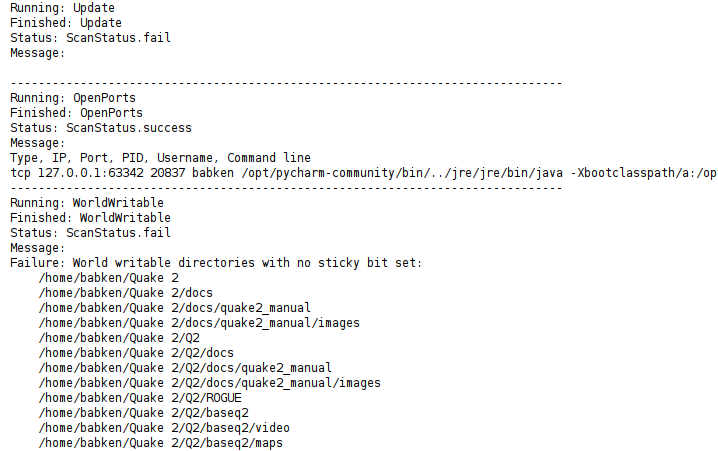
\includegraphics[width=1.0\textwidth]{result.png}
\end{figure}


\end{document}
